\documentclass[a4paper,12pt]{article}
\title{Washing the dishes to wash the dishes}
\author{Thich Nhat Hanh}
\usepackage{graphicx}
\begin{document}
 \maketitle
\begin{center}
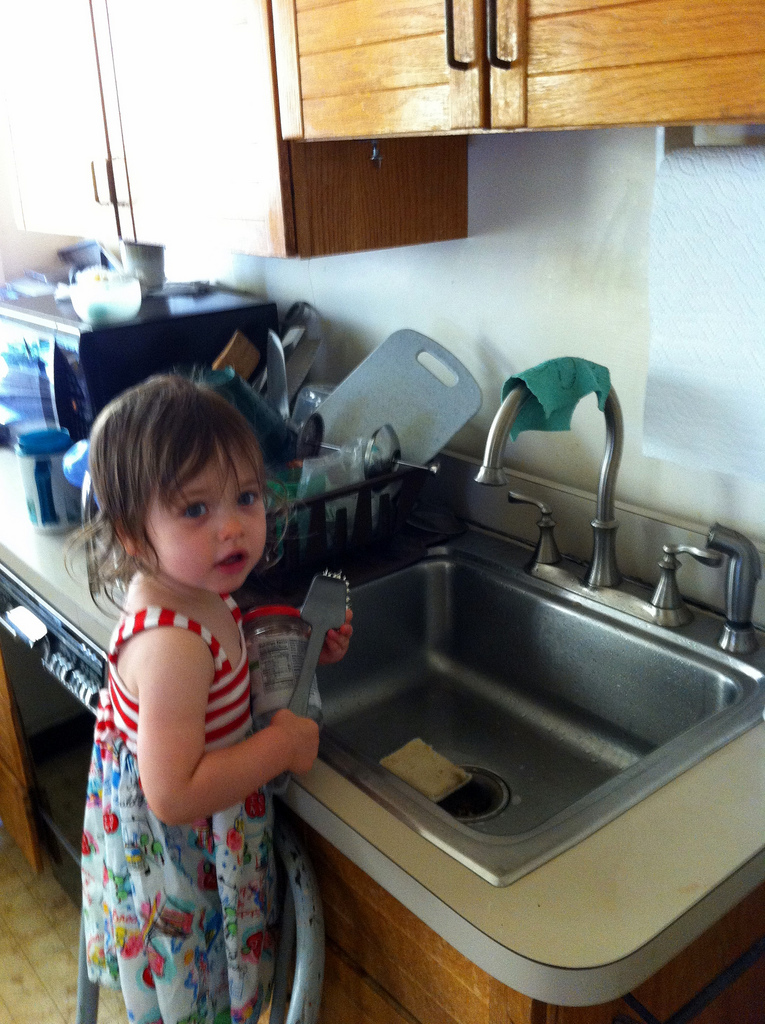
\includegraphics[scale=0.25]{washingdishes.jpg}
\end{center}
Thirty years ago, when I was still a novice at Tu Hieu Pagoda, washing the 
dishes was hardly a pleasant task. During the Season of Retreat when all the 
monks returned to the monastery, two novices had to do all the cooking and wash 
the dishes for sometimes well over one hundred monks.

There was no soap. We had only ashes, rice husks, and coconut husks, and that 
was all. Cleaning such a high stack of bowls was a chore, especially during the 
winter when the water was freezing cold. Then you had to heat up a big pot of 
water before you could do any scrubbing.

Nowadays one stands in a kitchen equipped with liquid soap, special scrubpads, 
and even running hot water which makes it all the more agreeable. It is easier 
to enjoy washing the dishes now. Anyone can wash them in a hurry, then sit down 
and enjoy a cup of tea afterwards. I can see a machine for washing clothes, 
although I wash my own things out by hand, but a dishwashing machine is going 
just a little too far!

While washing the dishes one should only be washing the dishes, which means that 
while washing the dishes one should be completely aware of the fact that one is 
washing the dishes. At first glance, that might seem a little silly: why put so 
much stress on a simple thing? But that’s precisely the point. The fact that I 
am standing there and washing these bowls is a wondrous 
reality. I'm being completely myself, following my breath, conscious of my 
presence and conscious of my thoughts and actions. There's no way I can be 
tossed around mindlessly like a bottle slapped here and there on the waves.


\paragraph{The cup in your hands :} There are two ways to wash the dishes. 
The first is to wash the dishes in order to have clean dishes and the second is 
to wash the dishes in order to wash the dishes. 

If while washing the dishes, we think only of the cup of tea that awaits us, 
thus hurrying to get the dishes out of the way as if they were a nuisance, then 
we are not ``washing the dishes to wash the dishes." What's more, we are not 
alive during the time we are washing the dishes.

In fact we are completely incapable of realizing the miracle of life while 
standing at the sink. If we can't wash the dishes, the chances are we won't be 
able to drink our tea either. While drinking the cup of tea, we will only be 
thinking of other things, barely aware of the cup in our hands. Thus we are 
sucked away into the future \--- and we are incapable of actually living one 
minute of life.
\end{document}
